% Compile from the manuscript root:
% latexmk -pdf -outdir=.verification/mixed-figures figures/MixedG.tex
% Copy the resulting MixedG.pdf beside this source for inclusion in main.tex.
\documentclass[tikz,border=4pt,11pt]{standalone}
\usepackage[T1]{fontenc}
\usepackage{lmodern}
\usepackage{amsmath}
\usetikzlibrary{arrows.meta}

\begin{document}
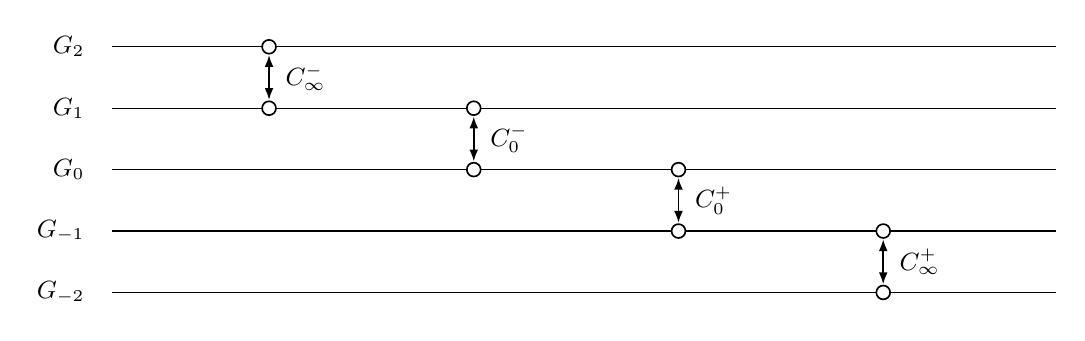
\begin{tikzpicture}[
    x=1cm,y=.78cm,font=\small,
    sheet/.style={line width=.45pt},
    exchange/.style={line width=.6pt,{Latex[length=1.5mm]}-{Latex[length=1.5mm]},
        shorten <=3pt,shorten >=3pt},
    endpoint/.style={circle,draw,line width=.6pt,fill=white,inner sep=0pt,
        minimum size=5pt},
    cut label/.style={fill=white,inner sep=1.5pt,anchor=west}
]
    % Sheet labels are exactly those of Appendix A.5.
    \foreach \index/\level in {2/4,1/3,0/2,-1/1,-2/0} {
        \draw[sheet] (0,\level) -- (12,\level);
        \node[anchor=east] at (-.22,\level) {$G_{\index}$};
    }

    % Each arrow is one sheet exchange over the named base-plane cut.
    % G exchange: C_infty^- (1,2).
    \draw[exchange] (2,3) -- (2,4);
    \node[cut label] at (2.15,3.5) {$C_\infty^-$};
    % G exchange: C_0^- (0,1).
    \draw[exchange] (4.6,2) -- (4.6,3);
    \node[cut label] at (4.75,2.5) {$C_0^-$};
    % G exchange: C_0^+ (0,-1).
    \draw[exchange] (7.2,1) -- (7.2,2);
    \node[cut label] at (7.35,1.5) {$C_0^+$};
    % G exchange: C_infty^+ (-1,-2).
    \draw[exchange] (9.8,0) -- (9.8,1);
    \node[cut label] at (9.95,.5) {$C_\infty^+$};

    \foreach \x/\y in {2/3,2/4,4.6/2,4.6/3,7.2/1,7.2/2,9.8/0,9.8/1}
        \node[endpoint] at (\x,\y) {};
\end{tikzpicture}
\end{document}
